% !TEX encoding = UTF-8 Unicode
\documentclass[a4paper,12pt]{report}
\usepackage[english,russian]{babel}
\usepackage[T1]{fontenc}
\usepackage[utf8]{inputenc}
\usepackage{indentfirst}
\usepackage{amsmath}
\usepackage{amssymb}
\usepackage{amsfonts}
\usepackage{bm}
\usepackage{setspace}
\usepackage{graphicx}
\usepackage{hyperref}
\usepackage{epstopdf}
\usepackage{graphicx}
\usepackage{algorithm,algorithmic}
\usepackage{caption}
\usepackage{subcaption}

\usepackage{geometry}
\geometry{left = 3cm}
\geometry{right = 1.5cm}
\geometry{top = 3cm}
\geometry{bottom = 3cm}

\DeclareMathOperator{\med}{med}

\renewcommand{\algorithmicrequire}{\textbf{Вход:}}
\renewcommand{\algorithmicensure}{\textbf{Выход:}}

\begin{document}
\title{Отчёт по заданию №2 \\ <<Поиск кратчайших путей между всеми вершинами графа>>}
\author{Зиннурова Э.А. \\ \textit{ВМК \, МГУ \, им. \, М.В. Ломоносова, кафедра ММП, 517 группа}}

\maketitle

\section*{Постановка задачи}
	\par Пусть нагруженный простой неориентированный граф $G=(V, E), |V| = n,$ задан своей матрицей смежности $A = (a_{ij})_{N \times N}$, т.е. 
	$$a_{ij} = \begin{cases}
		\text{вес $l(i,j) > 0$ ребра из вершины $i$ в вершину $j$, если таковое имеется},\\
		\infty \text{ иначе}.
		\end{cases}
$$
	\par Требуется с использованием модели MPI реализовать многопоточный алгоритм вычисления длин кратчайших путей между всеми парами вершин (в случае отсутствия пути между вершинами ответ полагается равным бесконечности) и вывода в формате списка рёбер с соответствующими длинами, провести его запуски на системах Lomonosov и Blue Gene/P, произвести замеры времени и проанализировать полученные результаты.
	
\section*{Описание последовательного алгоритма}
	\par Для решения поставленной задачи использовался алгоритм Флойда--Уоршелла.
	\par Пусть вершины графа пронумерованы от $1$ до $n$ и введено обозначение $d_{i j}^{k}$ для длины кратчайшего пути от вершины $i$ до $j$, который в качестве внутренних вершин включает только через вершины из множества $\{1 \ldots k\}$. Очевидно, что $d_{i j}^{0}$ — длина (вес) ребра $(i,\;j)$, если таковое существует.
	\par Для значения $d_{i j}^{k},\;k \in \mathbb (1,\;\ldots,\;n)$ возможны следующие варианты:
	\begin{enumerate}
	\item
	Кратчайший путь между вершинами $i$ и $j$ не проходит через вершину $k$, тогда $d_{i j}^{k}=d_{i j}^{k-1}$.
	\item
	Существует более короткий относительно $d_{ij}^{k-1}$ путь между вершинами $i$ и $j$, проходящий через вершину $k$. В данном случае он является конкатенацией кратчайших путей от вершины $i$ до $k$ и от $k$ до $j$, т.е. $d_{i j}^{k}=d_{i k}^{k-1} + d_{k j}^{k-1}.$
	\end{enumerate}

	\par Таким образом, имеем:
	$$d_{i j}^k = \begin{cases}
		a_{ij}, k =0,\\
		\min (d_{i j}^{k-1},\; d_{i k}^{k-1} + d_{k j}^{k-1}), k\ne 0.
		\end{cases}
$$

Алгоритм Флойда-Уоршелла последовательно вычисляет все значения $d_{i j}^{k}, \forall i,\; j, k = \overline{1,n}$. Значение $d_{ij}^n$ является длиной кратчайшего пути из вершину $i$ в $j$. 
\begin{algorithm}[H]
	\algorithmicrequire{N, $A$}\\
 	\algorithmicensure{$A'$}
	\begin{algorithmic}[1]
		\FOR{$k=1$ to $N$}
			\FOR{$i=1$ to $N$}
				\FOR{$j=1$ to $N$}
					\STATE $a_{ij} = \min(a_{ij}, a_{ik} + a_{kj})$
				\ENDFOR
			\ENDFOR
		\ENDFOR
	\end{algorithmic}
	\caption{Псевдокод алгоритма Флойда}
	\label{alg:seq}
\end{algorithm}

\section*{Описание параллельного алгоритма}
	\par Модифицируем описанный выше алгоритм. Как следует из общей схемы алгоритма Флойда, основная вычислительная нагрузка при решении задачи поиска кратчайших путей состоит в выполнении операции выбора минимальных значений. Данная операция является достаточно простой и ее распараллеливание не приведёт к заметному ускорению вычислений. Более эффективный способ организации параллельных вычислений может состоять в одновременном выполнении нескольких операций обновления значений матрицы $A$. 
	\par Формальный алгоритм распараллеливания по одной из размерностей матрицы $A$ приведён ниже.\\
\begin{minipage}{0.55\textwidth}
\begin{algorithm}[H]
	\algorithmicrequire{N, $A$}\\
 	\algorithmicensure{$A'$}
	\begin{algorithmic}[1]
		\FOR{$k=1$ to $N$}
			\FOR{$i=i_{\text{local start}}$ to $i_{\text{local end}}$}
				\FOR{$j=1$ to $N$}
					\STATE $a_{ij} = \min(a_{ij}, a_{ik} + a_{kj})$
				\ENDFOR
			\ENDFOR
		\ENDFOR
	\end{algorithmic}
	\caption{Распараллеливание по одной размерности матрицы $A$}
	\label{alg:seq}
\end{algorithm}
\end{minipage}
\begin{minipage}{0.4\textwidth}
\vspace{30pt}
\begin{figure}[H]
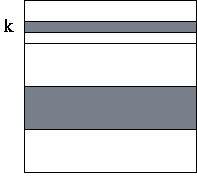
\includegraphics[width=0.8\textwidth]{./par1.png}
\end{figure}
\vspace{10pt}
\end{minipage}

\section*{Эксперименты}
	\par Проведём эксперименты для различных параметров числа потоков, тасков и узлов, измеряя время работы параллельной программы. Положим $N = 10^4$, матрицу $A$ будем генерировать следующим образом:
$$
a_{ij} = \begin{cases}
		\text{rand}(1000), p\\
		\infty, 1 - p,
		\end{cases}
$$
где $p$ --- вероятность образования ребра.\\
Поскольку сложность алгоритма зависит от $N = |V|,$ а не от $|E|,$ то большой роли значение $p$ не играет.
	\par На рис. \ref{lom} приведены графики, отражающие зависимости усреднённого по достаточно большому количеству запусков времени работы и ускорения от числа процессов для системы Lomonosov.
	
	\begin{figure}[H]
			\begin{subfigure}{0.5\textwidth}
				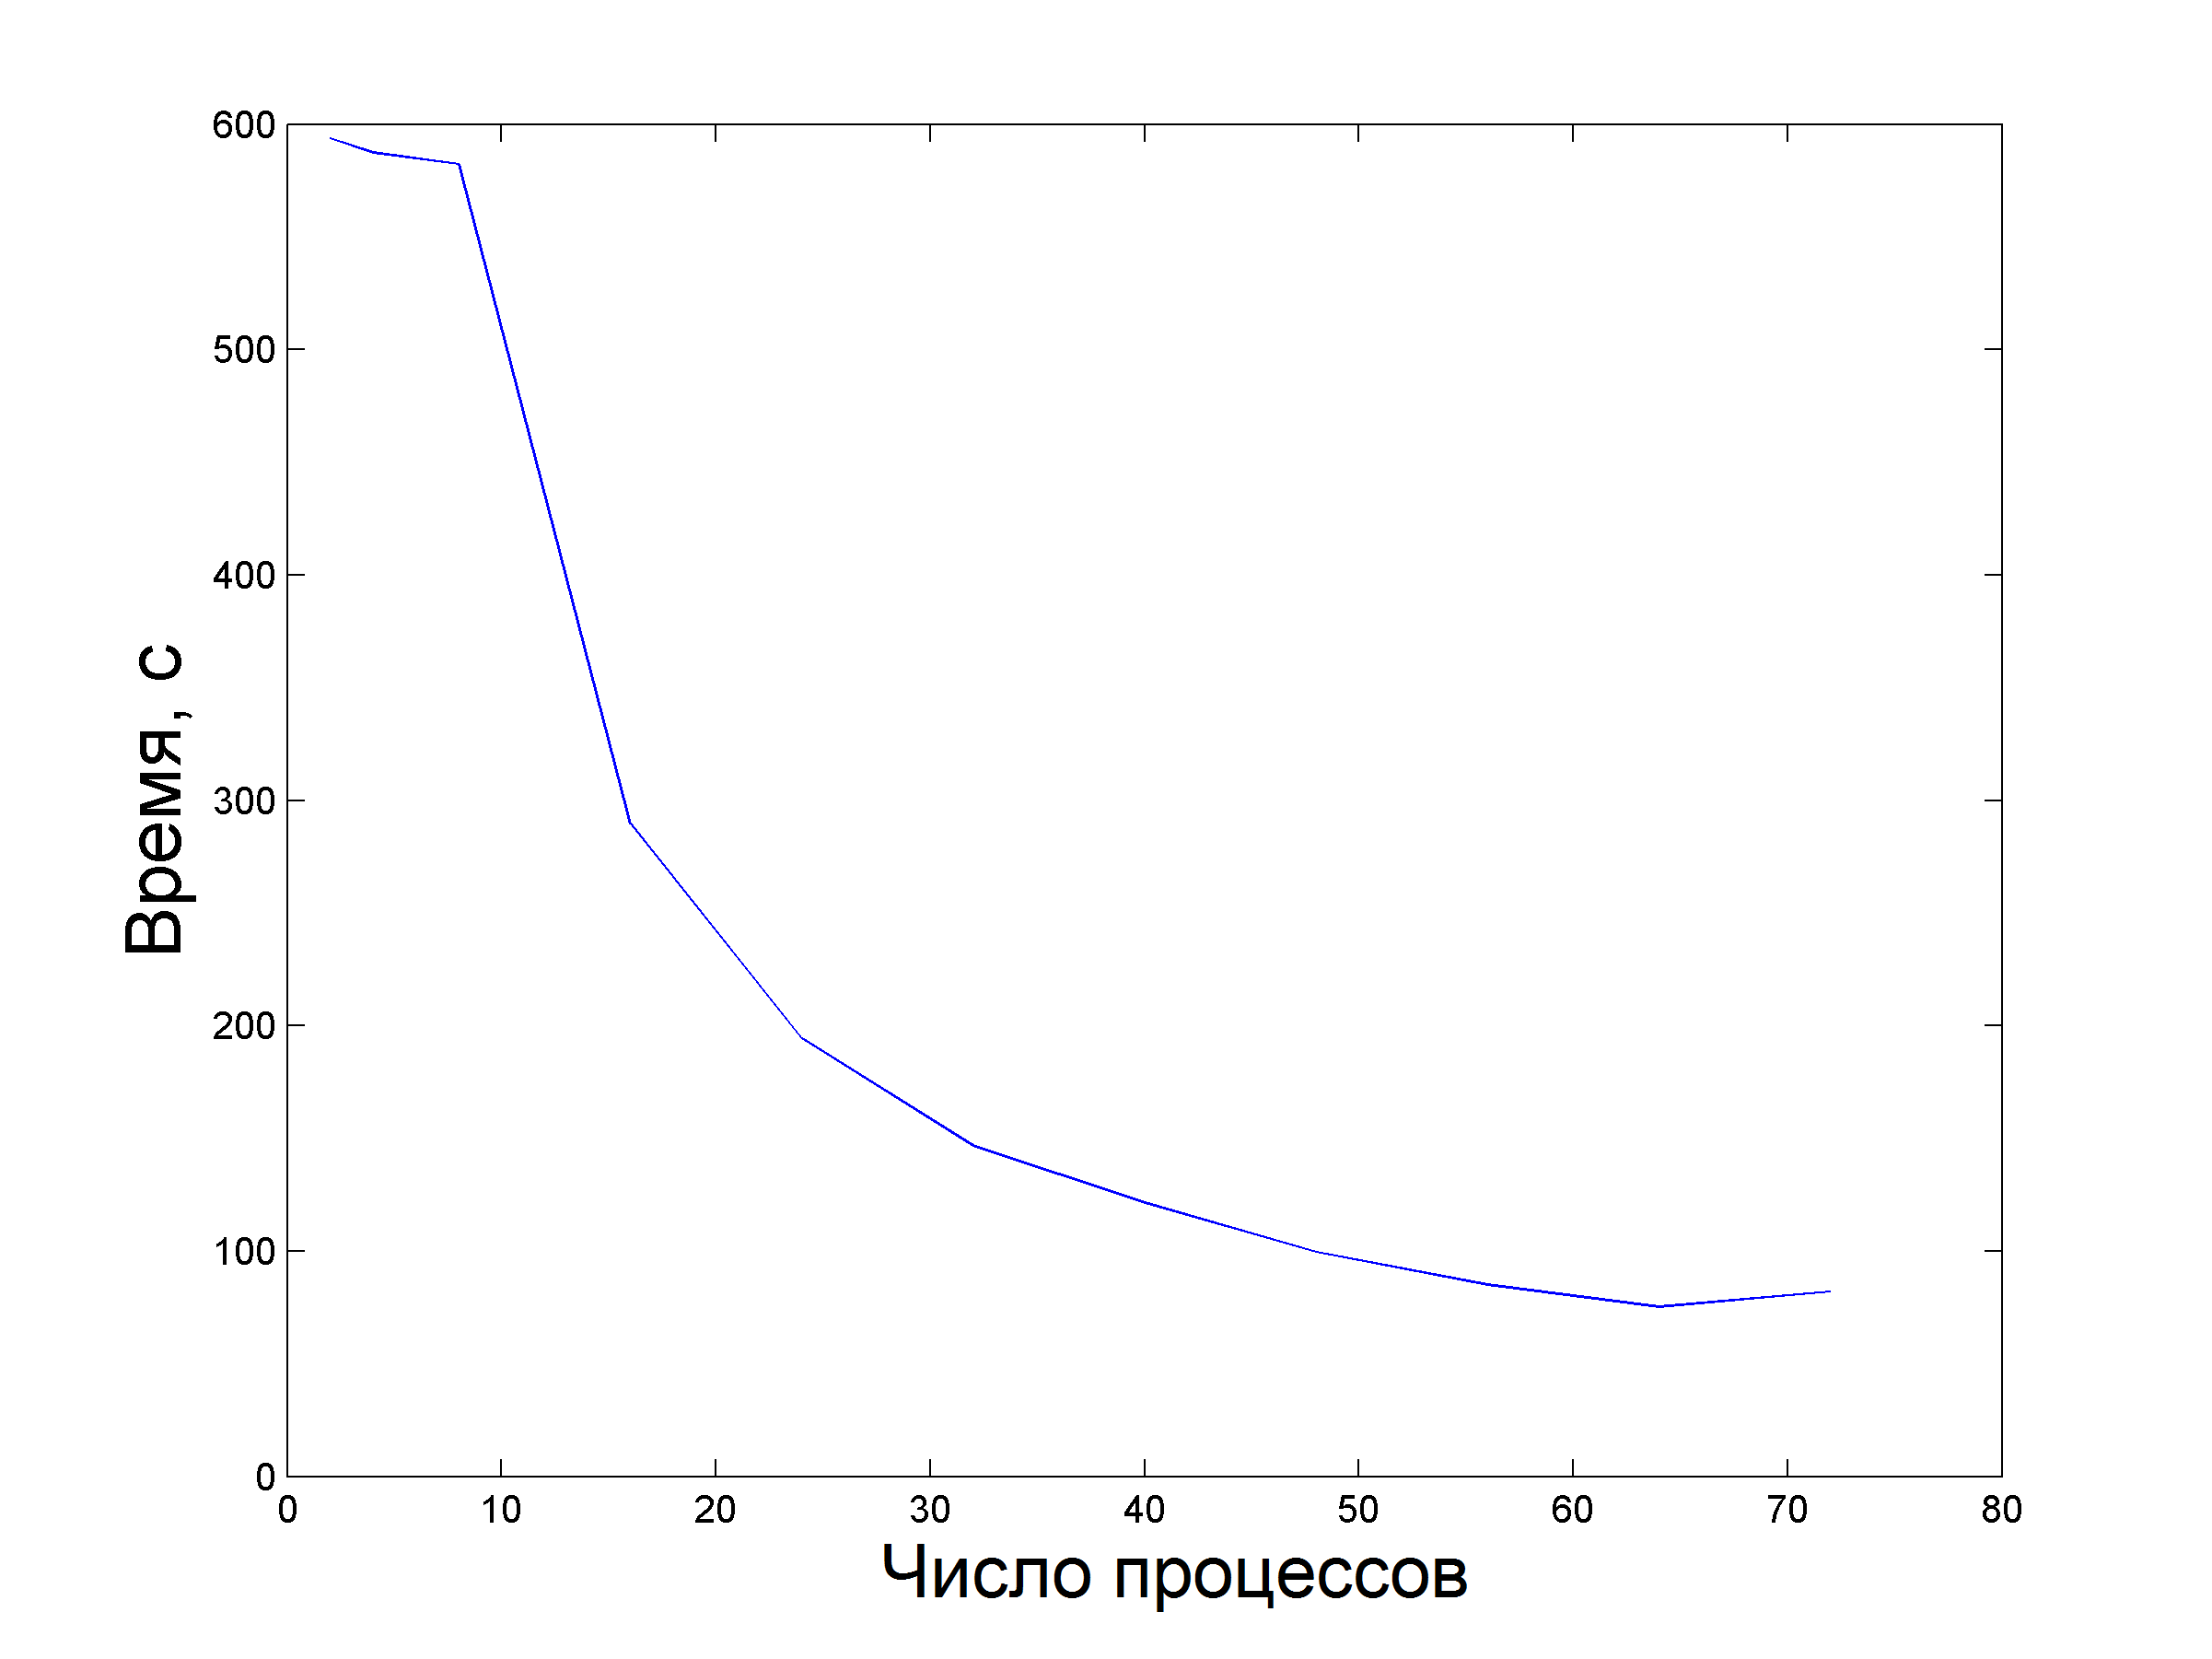
\includegraphics[width=\textwidth]{mpi_lom.png}
				\caption{Время выполнения}
			\end{subfigure}
			\begin{subfigure}{0.5\textwidth}
				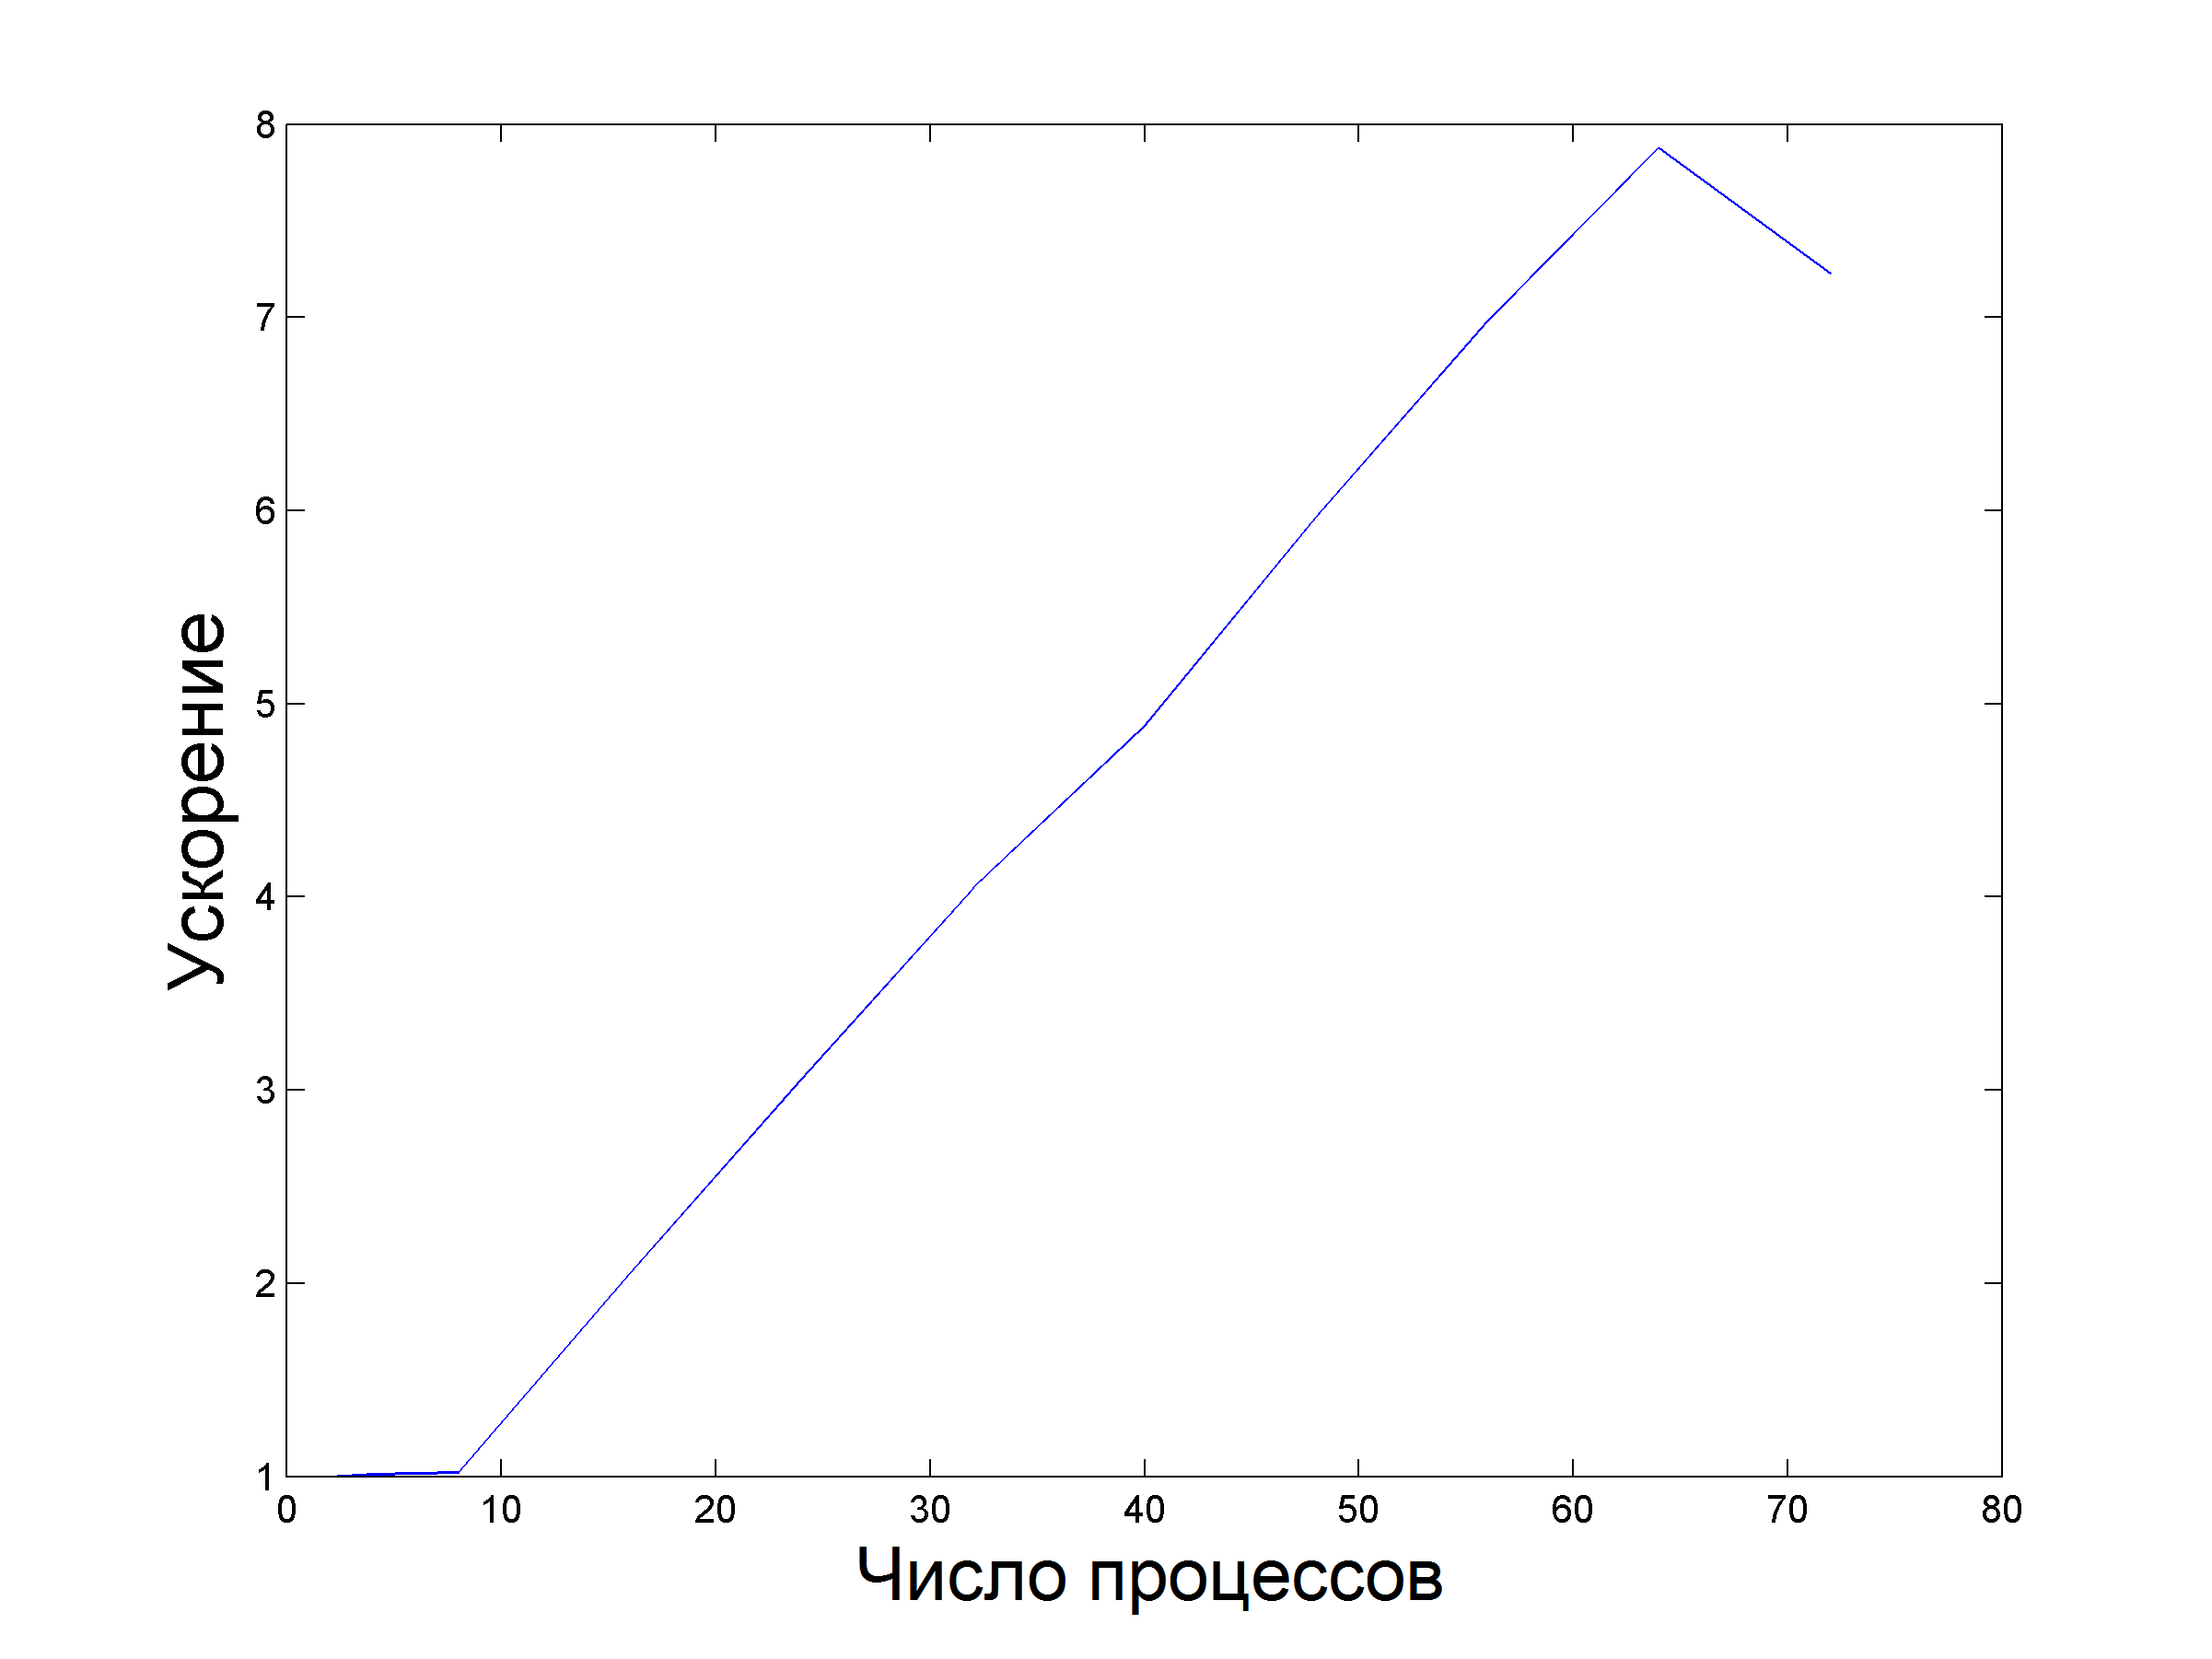
\includegraphics[width=\textwidth]{mpi_lom_speedup.png}
				\caption{Ускорение}
			\end{subfigure}
			\caption{Эксперименты на вычислительном комплексе «Ломоносов»}
			\label{lom}
		\end{figure}\par
	\par На рис. \ref{bg} приведены графики, отражающие зависимости усреднённого по достаточно большому количеству запусков времени работы и ускорения от числа процессов для системы Blue Gene/P.
	
	\begin{figure}[H]
			\begin{subfigure}{0.5\textwidth}
				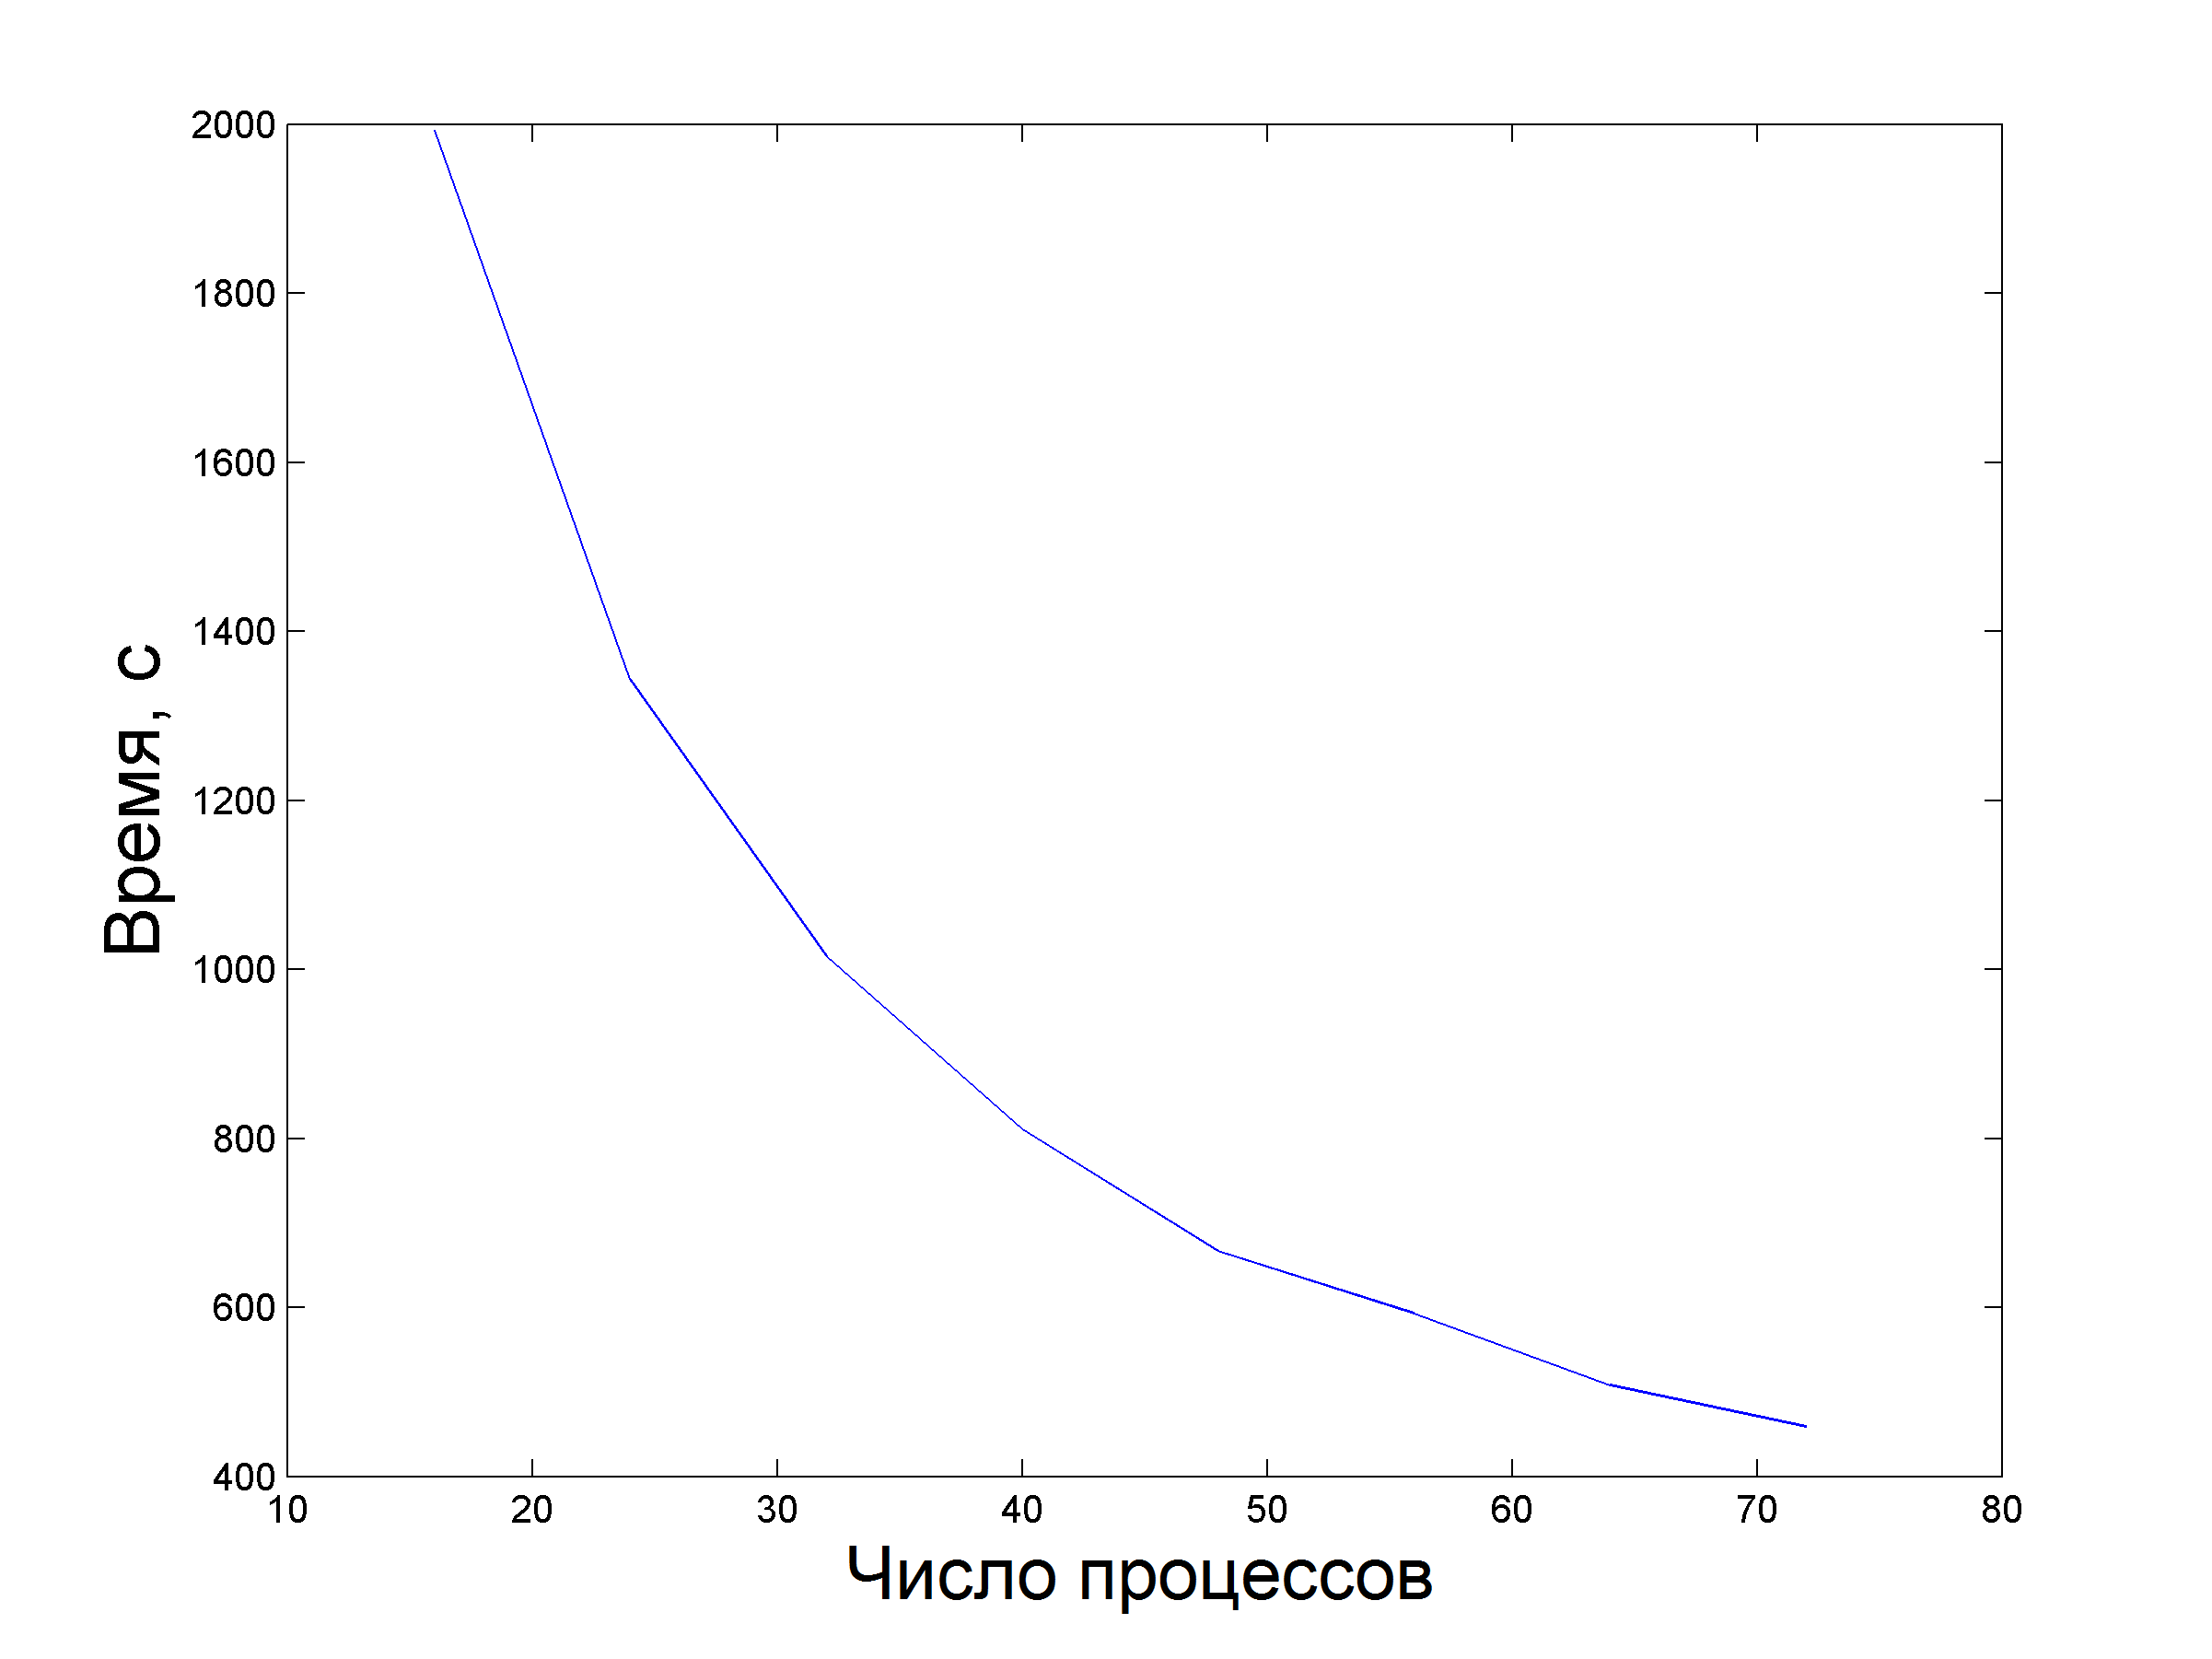
\includegraphics[width=\textwidth]{mpi_bg.png}
				\caption{Время выполнения}
			\end{subfigure}
			\begin{subfigure}{0.5\textwidth}
				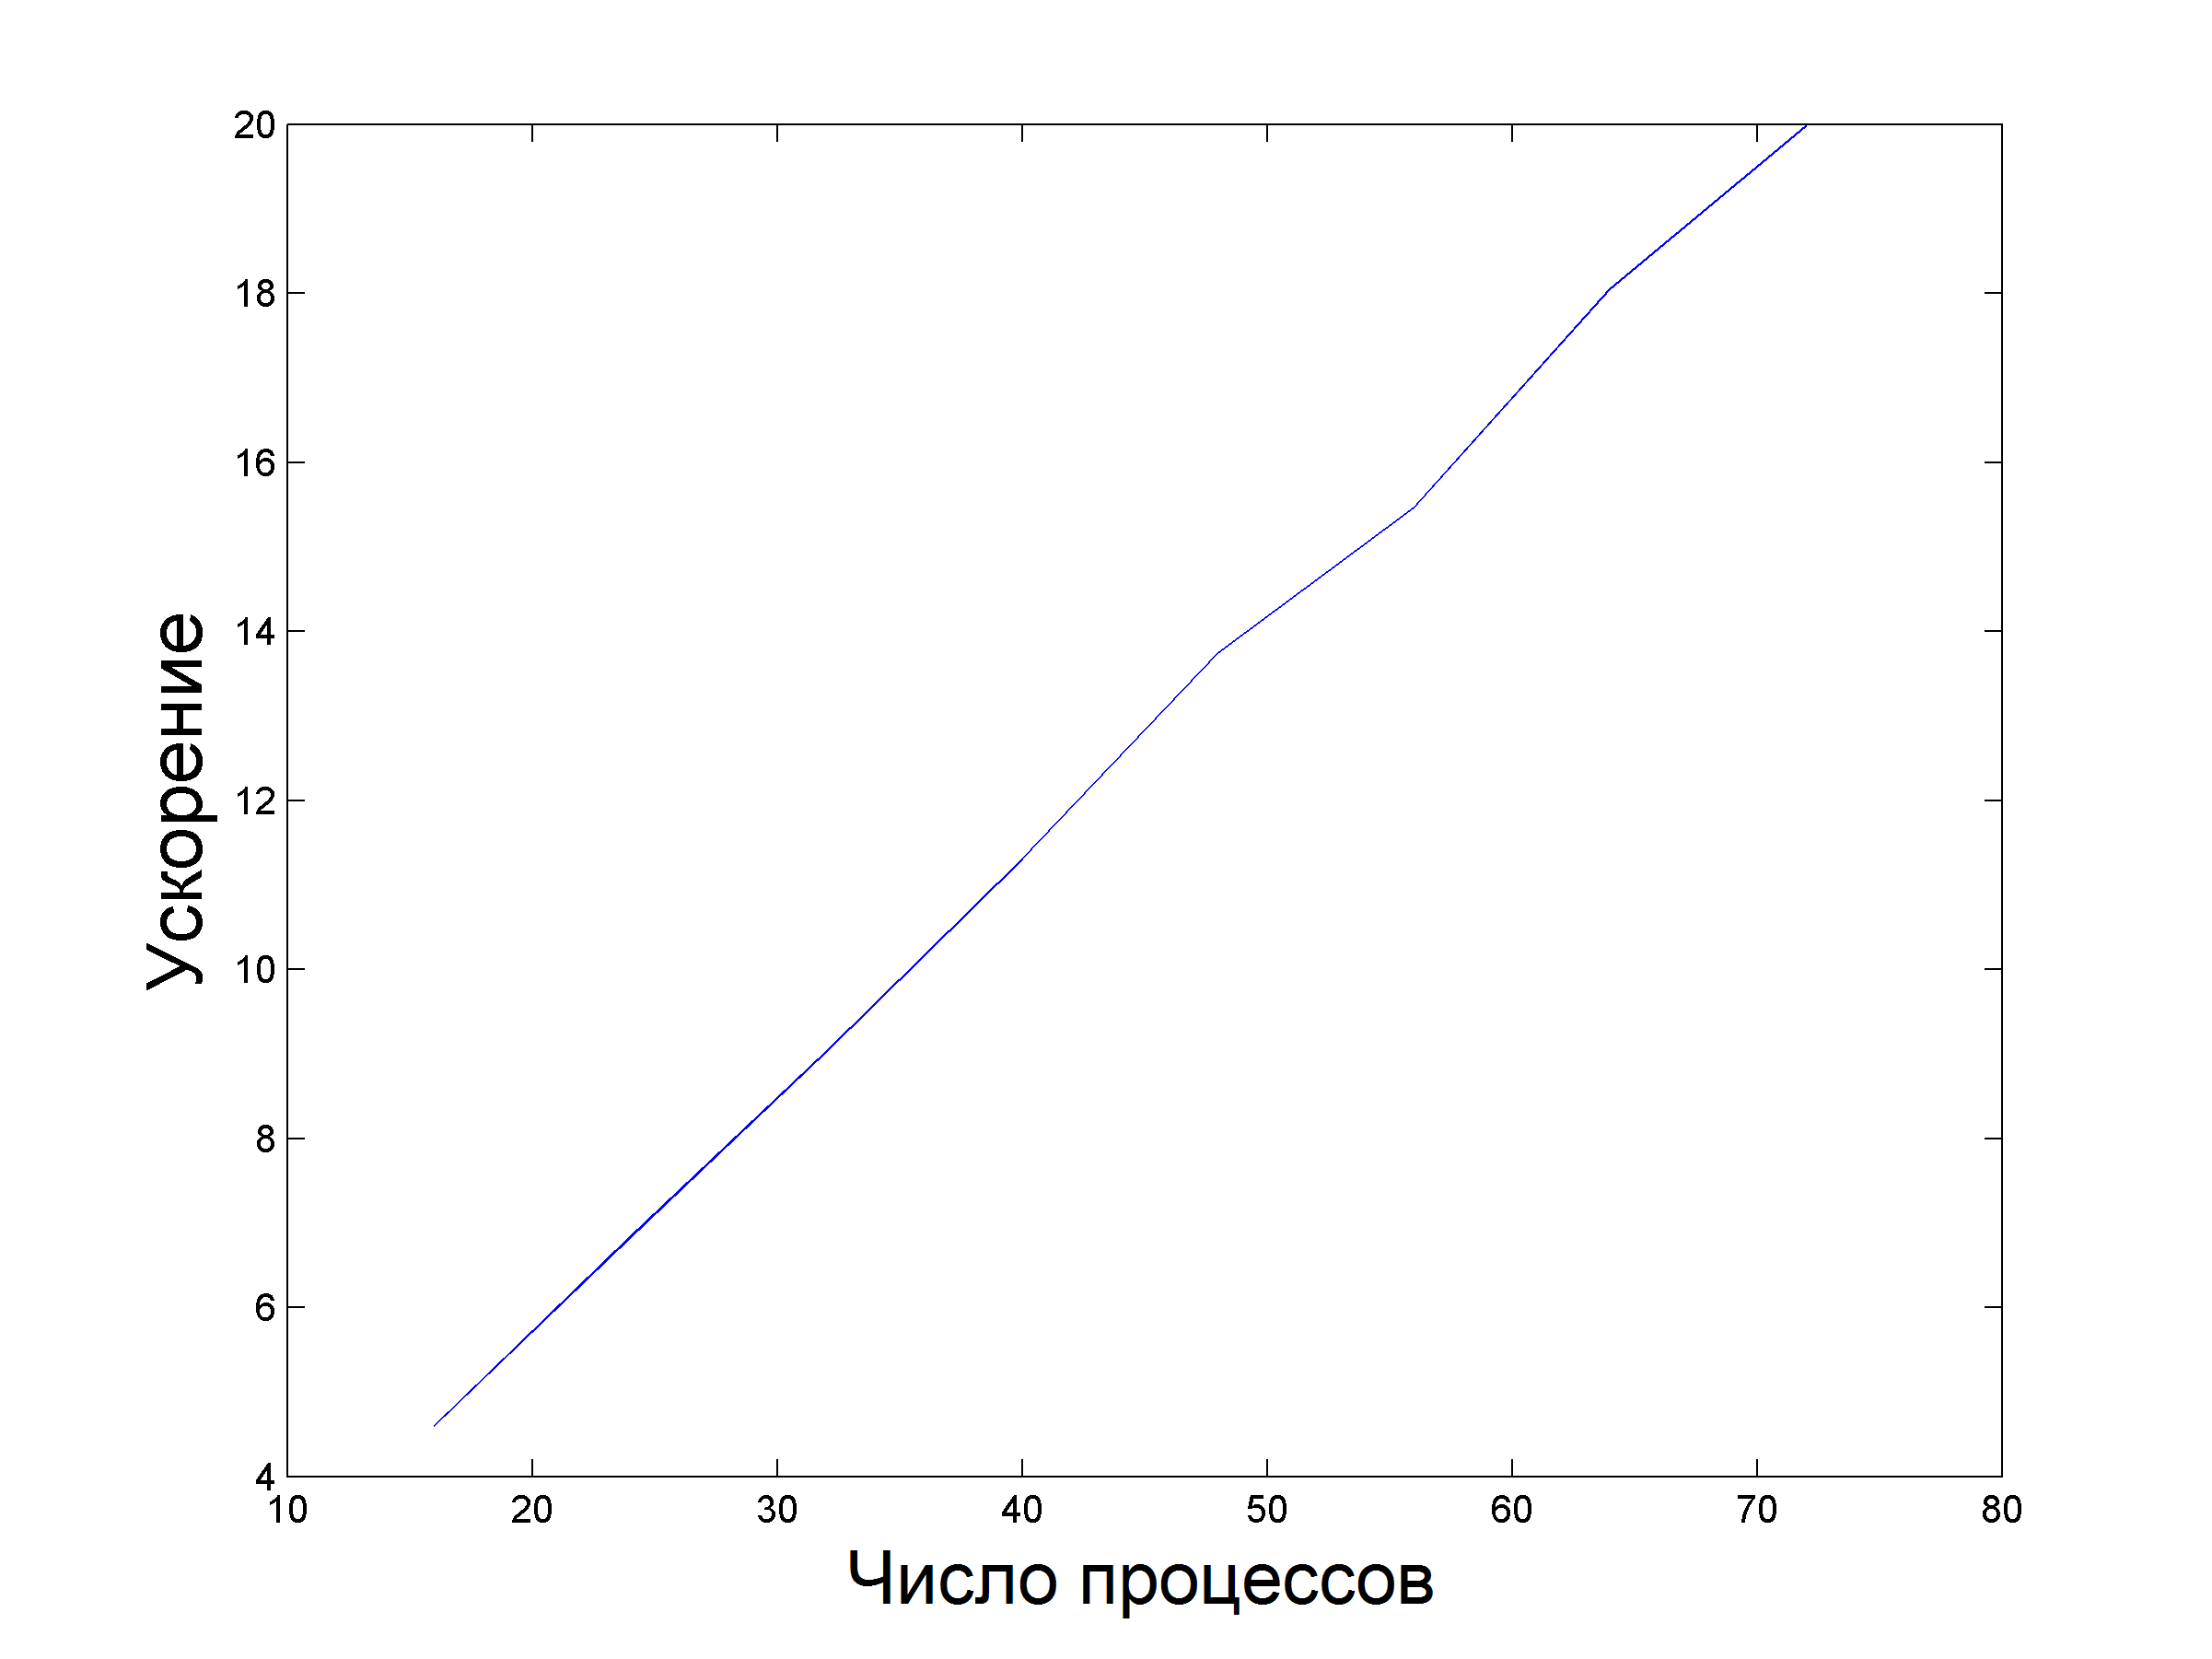
\includegraphics[width=\textwidth]{mpi_bg_speedup.png}
				\caption{Ускорение}
			\end{subfigure}
			\caption{Эксперименты на вычислительном комплексе BlueGene}
			\label{bg}
		\end{figure}\par


	\par Таким образом, легко видеть, что ускорение практически линейно зависит от числа процессов, что свидетельствует о  высокой масштабируемости рассматриваемой задачи.

\section*{Заключение}
	\par В рамках данного задания был реализован параллельный алгоритм вычисления кратчайших путей между всеми возможными парами вершин взвешенного графа, были проведены исследования эффективности распараллеливания данной задачи.
	
\section*{Список литературы}
\begin{enumerate}
\item
\href{http://www.mcs.anl.gov/~itf/dbpp/text/node35.html}{http://www.mcs.anl.gov/~itf/dbpp/text/node35.html}\\
\item
\href{http://www.academia.edu/243222/An\_Investigation\_Of\_Different\_Hybrid\_OpenMp\_and\_MPI\_Implementations\_Of\_Floyds\_All-Pairs-Shortest-Path\_Algorithm}{http://www.academia.edu/243222/An\_Investigation\_Of\_Different\_Hybrid\_OpenMp\_and\_MPI\_Implementations\_Of\_Floyds\_All-Pairs-Shortest-Path\_Algorithm}\\
\item
\href{http://www.hpcc.unn.ru/mskurs/RUS/DOC/ppr11.pdf}{http://www.hpcc.unn.ru/mskurs/RUS/DOC/ppr11.pdf}\\
%\href{http://ru.wikipedia.org/wiki/\%D0\%90\%D0\%BB\%D0\%B3\%D0\%BE\%D1\%80\%D0\%B8\%D1\%82\%D0\%BC\_\%D0\%A4\%D0\%BB\%D0\%BE\%D0\%B9\%D0\%B4\%D0\%B0\_\%E2\%80\%94\_\%D0\%A3\%D0\%BE\%D1\%80\%D1\%88\%D0\%B5\%D0\%BB\%D0\%BB\%D0\%B0}
\end{enumerate}

\end{document}
